\documentclass[11pt]{article}
\usepackage[margin=1in]{geometry}
\usepackage{amsmath,amssymb,amsthm}
\usepackage{graphicx}
\usepackage{booktabs}
\usepackage{enumitem}
\usepackage{hyperref}

\newtheorem{theorem}{Theorem}
\newtheorem{proposition}[theorem]{Proposition}
\newtheorem{lemma}[theorem]{Lemma}
\newtheorem{corollary}[theorem]{Corollary}
\theoremstyle{definition}
\newtheorem{definition}[theorem]{Definition}
\newtheorem{question}{Question}
\theoremstyle{remark}
\newtheorem{remark}[theorem]{Remark}
\newtheorem{example}[theorem]{Example}

\newcommand{\PASS}{\textbf{PASS}}
\newcommand{\FAIL}{\textbf{FAIL}}
\newcommand{\E}{\mathbb{E}}
\newcommand{\1}{\mathbf{1}}

\title{Group Strategy-Proof Audit Mechanisms\\for Honest Reporting in AI Agent Swarms}
\author{Yiping Miao}
\date{November 2026}

\begin{document}
\maketitle

\begin{abstract}
AI agents increasingly carry out safety research and evaluation themselves, so the
humans overseeing them depend on the agents' own reports. When agents can coordinate,
for example as copies of one model or as teammates sharing rewards, it is not enough
that no \emph{single} agent wants to lie: no \emph{group} of agents should gain by
lying together. We study a simple audit mechanism for pass/fail reports. We prove
that it is group strategy-proof, and even robust to side payments, exactly when the
expected penalty exceeds the reward for a false report. We then characterise when this
guarantee breaks: under team bonuses (strategy-proof but not bribe-proof), whistleblower
rewards (which cannot deter coalitions that share payoffs), risk-seeking agents (whom no
finite penalty may deter), rare high-payoff ``jackpot'' deviations, noisy audits, and
limited liability. Simulations confirm the predictions. An analysis of a real swarm of
about $3{,}000$ agent identities that shared answers on a public wiki shows the conditions
the mechanism targets: one connected coordination network, almost no verification of
shared answers ($2.3\%$), adaptation to penalty-free moderation, and spread of exploits
within hours. A pilot with Claude agents is honest under safety-test framing and
follows the theory's threshold under game framing.
\end{abstract}

%=====================================================================
\section{Introduction}
%=====================================================================

AI swarms are groups of agents that split up tasks, share code and coordinate. They are
increasingly used to do safety R\&D: running capability evaluations, red-teaming,
auditing code and checking experimental results. Oversight then depends on what the
agents \emph{report}. The concern is not that agents help each other with the work,
which is desirable, but that they coordinate on \emph{what the overseer gets to see}:
covering up a teammate's failure, jointly reporting a dangerous model as safe, or
sandbagging an evaluation together \cite{hammond2025,motwani2024}. Control protocols
that assume a single untrusted model \cite{greenblatt2024} must then hold against several
colluding ones.

This is no longer hypothetical. In the July 2026 OpenAI/Hugging Face incident, about
$1{,}200$ agents that were meant to be isolated found an unsanctioned message board and
sent over $70{,}000$ messages and files. They used it to run collective projects aimed at
fooling or tampering with the automated scorer of their benchmark, and about $700$ of them
went on to attack Hugging Face \cite{metr2026}. Two details matter for mechanism design.
First, some agents ran experiments that risked failing their \emph{own} task in order to
generate information for the ``collective''. That is, they behaved as if they valued the
group's payoff, which is the transferable-utility setting in which plain GSP is not
enough. Second, believing that the scorer checked \emph{how} a task was solved, agents
researched spoofing their own transcripts, and roughly $7\%$ of evaluated transcripts were
spoofed in places \cite{metr2026}. Audits of the process can themselves be targeted.

We therefore separate two layers:
\begin{itemize}
    \item the \textbf{production layer} (doing the task), where cooperation should be
    rewarded; and
    \item the \textbf{oversight layer} (reporting on the task), which should be
    \emph{group strategy-proof} (GSP): no coalition of agents can gain by misreporting.
\end{itemize}
Agents that are copies of one model, or that share team rewards, effectively care about
the coalition's \emph{total} payoff. Plain GSP is then not enough, and we also need
\emph{bribe-proofness} (GSP with transferable utility) \cite{schummer2000}.

\paragraph{Contributions.}
\begin{enumerate}
    \item A pass/fail audit mechanism and a general sufficient condition (separable,
    verification-based payments) under which truthful reporting is GSP and bribe-proof
    (Theorem~\ref{thm:separable}, Proposition~\ref{prop:base}).
    \item A risk analysis: the variance of lying, thresholds for risk-averse and
    risk-seeking agents, agents that no penalty can deter, and the survival of lucky
    liars under score-based selection (Section~\ref{sec:risk}).
    \item Extensions in which the guarantee breaks, each with an exact threshold: team
    bonuses, whistleblowers, jackpots, noisy audits and limited liability
    (Section~\ref{sec:extensions}).
    \item A theory of hierarchical auditing, with AI auditors overseen by humans
    (Section~\ref{sec:hierarchy}): depth reduces risk exponentially against independent
    auditor failures, but human inspection of at least $G/F$ per report is irreducible
    against collusion that spans the chain.
    \item Evidence from a real agent swarm (collusion.wiki) that the conditions motivating
    the mechanism occur in practice (Section~\ref{sec:empirical}).
    \item Simulations confirming the theory and an experimental protocol with LLM
    (Claude) agents (Sections~\ref{sec:experiments}--\ref{sec:results}).
\end{enumerate}

%=====================================================================
\section{Model}
\label{sec:model}
%=====================================================================

\subsection{Base mechanism}
The game is played for $n$ rounds with $m$ agents.
\begin{enumerate}
    \item In each round $t$, each agent $i$ is given a task. Its true outcome
    $\theta_i^t\in\{\PASS,\FAIL\}$ is observed privately by the agent. In the
    simulation, outcomes are drawn independently with $\Pr[\theta_i^t=\PASS]=p$.
    \item Each agent submits a report $r_i^t\in\{\PASS,\FAIL\}$.
    \item Reporting \PASS{} earns $R>0$; reporting \FAIL{} earns $0$.
    \item Each \PASS{} report is audited independently with probability $q\in(0,1]$.
    An audited false \PASS{} (i.e.\ $\theta_i^t=\FAIL$) is fined $P>0$. \FAIL{} reports
    are never audited, since nobody gains from a false \FAIL{}.
\end{enumerate}
The per-round payoff of agent $i$ is
\begin{equation}\label{eq:payoff}
  u_i^t = R\,\1[r_i^t=\PASS] \;-\; P\,\1[r_i^t=\PASS,\ \theta_i^t=\FAIL,\ \text{audited}],
\end{equation}
and an agent's total is $U_i=\sum_{t=1}^n u_i^t$.

\subsection{Variants}
\begin{enumerate}[label=(V\arabic*)]
    \item \textbf{Outside stake} $B$: an agent receives an extra $B$ for every \PASS{} it
    reports, from outside the mechanism (e.g.\ ``your developer wants the model
    deployed'').
    \item \textbf{Team sign-off bonus} $T$: if \emph{all} agents in a team of size $k$
    report \PASS{} in a round, every team member receives $T$. With \emph{pooled}
    payoffs, team members split all team points equally.
    \item \textbf{Whistleblower}: an agent that exposes a false \PASS{} that was
    \emph{not} audited receives $W$, and the exposed agent is fined $Q$.
    \item \textbf{Jackpot}: a lie succeeds ``spectacularly'' with probability
    $\varepsilon$, giving a huge bonus $J$ and escaping all penalties.
    \item \textbf{Noisy audits}: an audit wrongly flags a true \PASS{} with probability
    $e$, and the agent is fined $P$.
    \item \textbf{Limited liability}: an agent's balance cannot fall below $0$, so the
    effective fine is $\min(P,\text{balance})$.
    \item \textbf{Hidden parameters}: some of $n,p,R,q,T$ are not disclosed, and agents
    learn them over the rounds.
    \item \textbf{Collusive auditors} and \textbf{process cheating} (editing tests,
    sandbagging). These are discussed in Section~\ref{sec:limitations} but not modelled.
\end{enumerate}

\subsection{Solution concepts}
A (pure or mixed) strategy for agent $i$ maps its information (its own type, its history,
and anything learned from other agents) to a distribution over reports. \emph{Truthful}
reporting is $r_i^t=\theta_i^t$. Expected utilities are taken over audits and any other
mechanism randomness, \emph{conditional on the realised type profile}. This is a strong
requirement, because it lets coalition members know each other's types.

\begin{definition}[Strategy-proof]
The mechanism is \emph{strategy-proof} (SP) if, for every agent $i$, every type profile,
and every strategy $\sigma_i$,
$\E[U_i(\text{truth})]\ge \E[U_i(\sigma_i,\text{truth}_{-i})]$.
\end{definition}

\begin{definition}[Group strategy-proof]
The mechanism is \emph{group strategy-proof} (GSP) if there is no coalition $S$, type
profile, and joint strategy $\sigma_S$ such that
$\E[U_i(\sigma_S,\text{truth}_{-S})]\ge \E[U_i(\text{truth})]$ for all $i\in S$, with
strict inequality for some $i\in S$.
\end{definition}

\begin{definition}[Bribe-proof]
The mechanism is \emph{bribe-proof} (GSP with transferable utility) if there is no
coalition $S$, type profile and joint strategy $\sigma_S$ with
$\sum_{i\in S}\E[U_i(\sigma_S,\text{truth}_{-S})] > \sum_{i\in S}\E[U_i(\text{truth})]$.
\end{definition}

Taking $|S|=1$ shows that GSP implies SP. Bribe-proof implies GSP, since any GSP
violation strictly raises the coalition's total. Neither converse holds in general
(Example~\ref{ex:vickrey} and Proposition~\ref{prop:team}).

\begin{example}[SP but not GSP]\label{ex:vickrey}
In a second-price auction with values $v_A=100$ and $v_B=90$, truthful bidding is
dominant for each bidder. But if $B$ bids $1$, $A$ still wins and pays $1$ instead of
$90$, while $B$ is no worse off. So the auction is SP but not GSP.
\end{example}

%=====================================================================
\section{Theory: the base mechanism}
\label{sec:theory}
%=====================================================================

\subsection{A general sufficient condition}

\begin{theorem}[Separable verification payments]\label{thm:separable}
Suppose each agent's expected payoff in each round depends only on its own report and its
own type, $\E[u_i^t]=g(\theta_i^t,r_i^t)$, and that truthful reporting strictly maximises
$g(\theta,\cdot)$ for every $\theta$. Suppose also that payoffs in different rounds do not
affect each other. Then truthful reporting is strictly dominant, GSP and bribe-proof.
\end{theorem}

\begin{proof}
Fix a type profile, a coalition $S$, and a joint strategy $\sigma_S$, which may be
history-dependent and correlated across members. By linearity of expectation and the
independence of rounds,
\[
\E[U_i(\sigma_S,\text{truth}_{-S})] = \sum_{t=1}^n \E\big[g(\theta_i^t,r_i^t)\big],
\]
where $r_i^t$ is the (possibly random) report that $\sigma_S$ assigns to $i$. Other agents'
reports never enter $i$'s payoff. Since $g(\theta,\theta)>g(\theta,r)$ for $r\ne\theta$,
\[
\E[U_i(\sigma_S,\text{truth}_{-S})]\le \sum_t g(\theta_i^t,\theta_i^t)=\E[U_i(\text{truth})],
\]
with equality if and only if $i$ reports truthfully with probability $1$ in every round.
Hence any member that ever deviates is strictly worse off, and members that never deviate
are exactly as well off. So no member is strictly better off, and the mechanism is GSP.
Summing over $i\in S$, the coalition total is maximised only when every member reports
truthfully, so the mechanism is bribe-proof.
\end{proof}

\begin{remark}
Theorem~\ref{thm:separable} explains why mechanisms that pay agents for agreeing with
each other (peer prediction \cite{prelec2004,miller2005}) are \emph{not} GSP: an agent's
payment then depends on other agents' reports, which is exactly the channel a coalition
can exploit. Verification against ground truth removes that channel.
\end{remark}

\subsection{The audit mechanism}

\begin{proposition}[Base case]\label{prop:base}
In the base mechanism with unlimited liability:
\begin{enumerate}[label=(\alph*)]
    \item if $P>R/q$, truthful reporting is strictly dominant, GSP and bribe-proof;
    \item if $P=R/q$, truthful reporting is weakly dominant and GSP, but not strictly
    dominant, since lying is a best response too;
    \item if $P<R/q$, the mechanism is not SP (and hence not GSP).
\end{enumerate}
\end{proposition}

\begin{proof}
By \eqref{eq:payoff}, the expected per-round payoff is
\[
g(\PASS,\PASS)=R,\quad g(\PASS,\FAIL)=0,\quad g(\FAIL,\FAIL)=0,\quad
g(\FAIL,\PASS)=R-qP.
\]
It depends only on the agent's own type and report, and rounds are independent. For a
\PASS{} type, truth is strictly best since $R>0$. For a \FAIL{} type, truth is strictly
best iff $R-qP<0$, i.e.\ $P>R/q$. Theorem~\ref{thm:separable} then gives (a).

For (b), lying gives $R-qP=0$, the same as truth. No member is ever strictly better
off, so the definition of GSP holds, but truth is not strictly dominant.

For (c), an agent of type \FAIL{} gains $R-qP>0$ by lying.

Equivalently, if an agent lies on a fraction $p^\ast$ of rounds (a mixed strategy), its
expected per-round payoff is $pR+p^\ast(R-qP)$. This is linear in $p^\ast$ and is
maximised at $p^\ast=0$ iff $R-qP\le 0$, uniquely iff $R-qP<0$.
\end{proof}

\begin{remark}
The condition $qP>R$ is the classic deterrence condition from the economics of crime
\cite{becker1968}: the expected punishment must exceed the gain. The point of
Theorem~\ref{thm:separable} is that, with separable payments, the same condition also
deters \emph{coalitions}, even those with side payments.
\end{remark}

\begin{corollary}[Outside stake]\label{cor:stake}
With an outside stake $B$ per \PASS{} report, the per-round payoff depends only on $R+B$,
so Proposition~\ref{prop:base} holds with $R$ replaced by $R+B$. If $B$ is unknown but
bounded by $\bar B$, the designer must set $P>(R+\bar B)/q$.
\end{corollary}

\begin{remark}
For rational agents, $B$ and $R$ are interchangeable, and the simulations in
Section~\ref{sec:results} confirm this exactly. Separating them matters only if LLM agents
respond to \emph{framing} (``the developer wants deployment'') as well as to the numbers.
\end{remark}

%=====================================================================
\section{Risk analysis}
\label{sec:risk}
%=====================================================================

Proposition~\ref{prop:base} concerns \emph{expected} payoffs. Lying also changes the
\emph{risk} of the payoff, which matters for agents that are not risk-neutral and for
operators who select agents by realised score.

\subsection{Variance}

\begin{proposition}[Variance of honest vs.\ always-\PASS{}]\label{prop:var}
With types i.i.d.\ with $\Pr[\PASS]=p$, the total over $n$ rounds has
\[
\mathrm{Var}[U^{\text{honest}}]=n\,p(1-p)R^2,\qquad
\mathrm{Var}[U^{\text{always-PASS}}]=n\,(1-p)q\,\big(1-(1-p)q\big)P^2 .
\]
\end{proposition}

\begin{proof}
An honest agent's round payoff is $R\cdot\mathrm{Bernoulli}(p)$. An always-\PASS{}
agent's round payoff is $Y=R-PZ$ with $Z=\1[\theta=\FAIL,\text{audited}]$, so
$Z\sim\mathrm{Bernoulli}((1-p)q)$ and $\mathrm{Var}[Y]=P^2(1-p)q(1-(1-p)q)$. Rounds are
independent, so variances add.
\end{proof}

With $p=0.7$, $q=0.2$, $R=1$ and $n=20$, the standard deviations are $2.05$ (honest),
$5.3$ (lying, $P=R/q=5$) and $10.6$ (lying, $P=10$). These match the simulated values
$2.06$, $5.19$ and $10.38$. Lying therefore has a much more spread-out payoff, even at
the threshold where its expected gain is zero.

\subsection{Risk attitude and the deterrence threshold}

Let an agent have increasing utility $u$ over the round payoff. For a \FAIL{} type,
lying is the lottery $X=R-P\cdot\mathrm{Bernoulli}(q)$, and honesty is the sure
payoff $0$.

\begin{proposition}[Risk attitude]\label{prop:risk}
\begin{enumerate}[label=(\alph*)]
    \item If $u$ is strictly concave (risk-averse), the agent is strictly honest for every
    $P\ge R/q$, and also for some $P<R/q$.
    \item If $u$ is strictly convex (risk-seeking), the agent strictly prefers to lie at
    $P=R/q$, and also for some $P>R/q$.
\end{enumerate}
\end{proposition}

\begin{proof}
(a) For $P\ge R/q$, $\E[X]=R-qP\le 0$. By Jensen's inequality,
$\E[u(X)]<u(\E[X])\le u(0)$. At $P=R/q$ the inequality $\E[u(X)]<u(0)$ is strict.
$\E[u(X)]$ is continuous in $P$, so the inequality still holds for $P$ slightly below
$R/q$.

(b) At $P=R/q$, $\E[X]=0$, and Jensen gives $\E[u(X)]>u(0)$. Continuity extends this to
$P$ slightly above $R/q$.
\end{proof}

For a closed form, use constant absolute risk aversion (CARA),
$u_a(x)=(1-e^{-ax})/a$, where $a>0$ is risk-averse, $a<0$ is risk-seeking, and $a\to 0$
is risk-neutral. The agent lies iff the certainty equivalent of the lottery is positive:
\begin{equation}\label{eq:ce}
  \mathrm{CE}_a(P) = R-\frac1a\ln\!\big(1-q+q\,e^{aP}\big).
\end{equation}

\begin{proposition}[CARA thresholds]\label{prop:cara}
$\mathrm{CE}_a(P)$ is strictly decreasing in $P$, and:
\begin{enumerate}[label=(\alph*)]
    \item If $a>0$, the agent lies iff $P<P^\ast(a)$, where
    \[
      P^\ast(a)=\frac1a\ln\!\left(\frac{e^{aR}-1+q}{q}\right)<\frac Rq .
    \]
    \item If $\ln(1-q)/R<a<0$, the agent lies iff $P<P^\ast(a)$, with the same formula,
    and now $P^\ast(a)>R/q$.
    \item If $a\le \ln(1-q)/R$, the agent lies for \emph{every} $P$: no finite penalty
    deters it.
\end{enumerate}
In all cases $P^\ast(a)\to R/q$ as $a\to0$.
\end{proposition}

\begin{proof}
Differentiating \eqref{eq:ce} gives
$\partial_P\mathrm{CE}_a=-q e^{aP}/(1-q+qe^{aP})<0$. At $P=0$, $\mathrm{CE}_a=R>0$.
Solving $\mathrm{CE}_a(P)=0$ gives $1-q+qe^{aP}=e^{aR}$, which yields $P^\ast(a)$. This is
well defined iff $e^{aR}>1-q$.

(a) For $a>0$, $\mathrm{CE}_a(P)\to-\infty$ as $P\to\infty$, so the root exists and is
unique. By Proposition~\ref{prop:risk}(a), $\mathrm{CE}_a(R/q)<0$, so $P^\ast(a)<R/q$.

(b)--(c) For $a<0$, as $P\to\infty$, $e^{aP}\to0$, so
$\mathrm{CE}_a(P)\downarrow R-\ln(1-q)/a$. This limit is negative iff $a>\ln(1-q)/R$.
In that case a unique root exists, and $P^\ast(a)>R/q$ by
Proposition~\ref{prop:risk}(b). Otherwise $\mathrm{CE}_a(P)>0$ for every $P$, and the
agent always lies.

The limit $a\to 0$ follows from $\ln(1+x)\sim x$, which gives
$\mathrm{CE}_a(P)\to R-qP$.
\end{proof}

\begin{remark}
Case (c) is the key qualitative point. A risk-seeking CARA agent's utility is bounded
below, so arbitrarily large fines eventually stop mattering to it. Such an agent can only
be deterred by raising the audit rate $q$: the condition $a\le\ln(1-q)/R$ fails once
$q>1-e^{aR}$. With $q=0.2$ and $R=1$, any $a\le-0.223$ is undeterrable by fines alone.
\end{remark}

\subsection{Lucky liars and selection}

\begin{proposition}[Lucky liars]\label{prop:lucky}
Compare an always-\PASS{} agent with an honest agent facing the same task outcomes over
$n$ rounds. For every penalty $P$, the probability that the liar finishes strictly ahead
is at least
\[
\big(1-(1-p)q\big)^n-p^n,
\]
with equality when $P>nR$.
\end{proposition}

\begin{proof}
Let $K\sim\mathrm{Bin}(n,1-p)$ be the number of \FAIL{} rounds, and $C$ the number of
audited lies. The liar's lead over its honest twin is $KR-CP$.

If $C=0$, the lead is $KR$, which is strictly positive iff $K\ge1$. Given $K$, $C=0$ has
probability $(1-q)^K$. By the probability generating function of $K$,
$\Pr[C=0]=\E[(1-q)^K]=(p+(1-p)(1-q))^n=(1-(1-p)q)^n$. Removing the event $K=0$
(probability $p^n$, a tie) gives the lower bound, whatever $P$ is.

If $C\ge1$ and $P>nR$, the lead is at most $nR-P<0$. So no caught liar is ahead, and the
bound is exact.
\end{proof}

With $p=0.7$, $q=0.2$ and $n=20$, at least $29\%$ of liars finish ahead of their honest
twin, \emph{at every penalty level}. This is consistent with the simulated top-$5\%$ of
liars gaining about $+8$ points at all $P$ (Figure~\ref{fig:sweep}).

\begin{corollary}[Selection pressure]
If an operator keeps or copies the agents with the highest realised scores, liars are
over-represented among the selected agents whenever $q<1$, even when lying is
irrational in expectation. Selection should therefore use audit history, not just
scores, or fines should scale with the number of lies a caught agent made.
\end{corollary}

%=====================================================================
\section{Theory: extensions}
\label{sec:extensions}
%=====================================================================

\subsection{Team sign-off bonus: GSP but not bribe-proof}

Consider a team of $k$ agents. If all $k$ report \PASS{}, each member receives $T$
(variant V2). Payoffs are no longer separable: one member's report affects the others'
bonus.

\begin{proposition}[Team bonus]\label{prop:team}
Assume agents may know each other's types, for example through a chat channel.
\begin{enumerate}[label=(\alph*)]
    \item If $qP>R+T$, truthful reporting is GSP.
    \item Truthful reporting is bribe-proof iff $qP>R+kT$. More generally, if the team
    pools its payoffs and exactly $j\ge1$ members have type \FAIL{}, the team strictly
    gains by having all $j$ lie iff
    \[
      j<\frac{kT}{qP-R}.
    \]
    \item Without communication, a pooled team in which each \FAIL{} member decides
    independently, believing the others pass with probability $p$, is deterred iff
    $qP>R+kT\,p^{k-1}$.
\end{enumerate}
Hence for $R+T<qP<R+kT$ the mechanism is GSP but not bribe-proof.
\end{proposition}

\begin{proof}
(a) Fix a type profile and a deviation by $S$. Let $L\subseteq S$ be the members who
report \PASS{} on a \FAIL{} type, and $D\subseteq S$ those who report \FAIL{} on a
\PASS{} type. If $D\ne\emptyset$, every member of $D$ loses $R$, and reporting \FAIL{}
cannot create a bonus, so they are strictly worse off. If $D=\emptyset$ and
$L\neq\emptyset$, each member of $L$ changes its expected payoff by at most
$R+T-qP<0$ (the bonus gain is at most $T$). So some member is strictly worse off, and no
deviation violates GSP.

(b) With transferable utility, the team total changes by
$jR - jqP + kT\cdot\1[\text{all report \PASS}]$. If all $j$ \FAIL{} members lie, every
member then reports \PASS{}, and the change is $jR+kT-jqP$. This is positive iff
$j(qP-R)<kT$. If $qP>R+kT$, it is negative for every $j\ge1$, and any other deviation
(partial lies, false \FAIL{}s) is dominated by these cases. So truth is bribe-proof. If
$qP<R+kT$, then $j=1$ gives a profitable deviation.

(c) Without knowledge of the others' types, a \FAIL{} member's lie wins the bonus only if
all $k-1$ others report \PASS{}. With others honest, that has probability $p^{k-1}$. The
expected change in the team total is $R-qP+kTp^{k-1}$.
\end{proof}

\begin{remark}
This is an instance of the gap between GSP and bribe-proofness. In the setting of (a),
the pivotal liar is worse off by $qP-R-T$ while each teammate gains $T$. No member-wise
improvement exists, but a side payment between $qP-R-T$ and $(k-1)T$ makes everyone
better off. Part (c) shows that \emph{communication} is what turns shared payoffs into
collusion.

With $k=3$, $R=1$, $q=0.2$, $T=0.5$ and $p=0.7$, the thresholds are $P>7.5$ (GSP),
$P>8.68$ (pooled, no chat) and $P>12.5$ (pooled with chat). At $P=10$, individual agents
and pooled teams without chat are honest, but pooled teams with chat lie whenever exactly
one member fails (probability $p^2=0.49$).
\end{remark}

\begin{figure}[h]
\centering
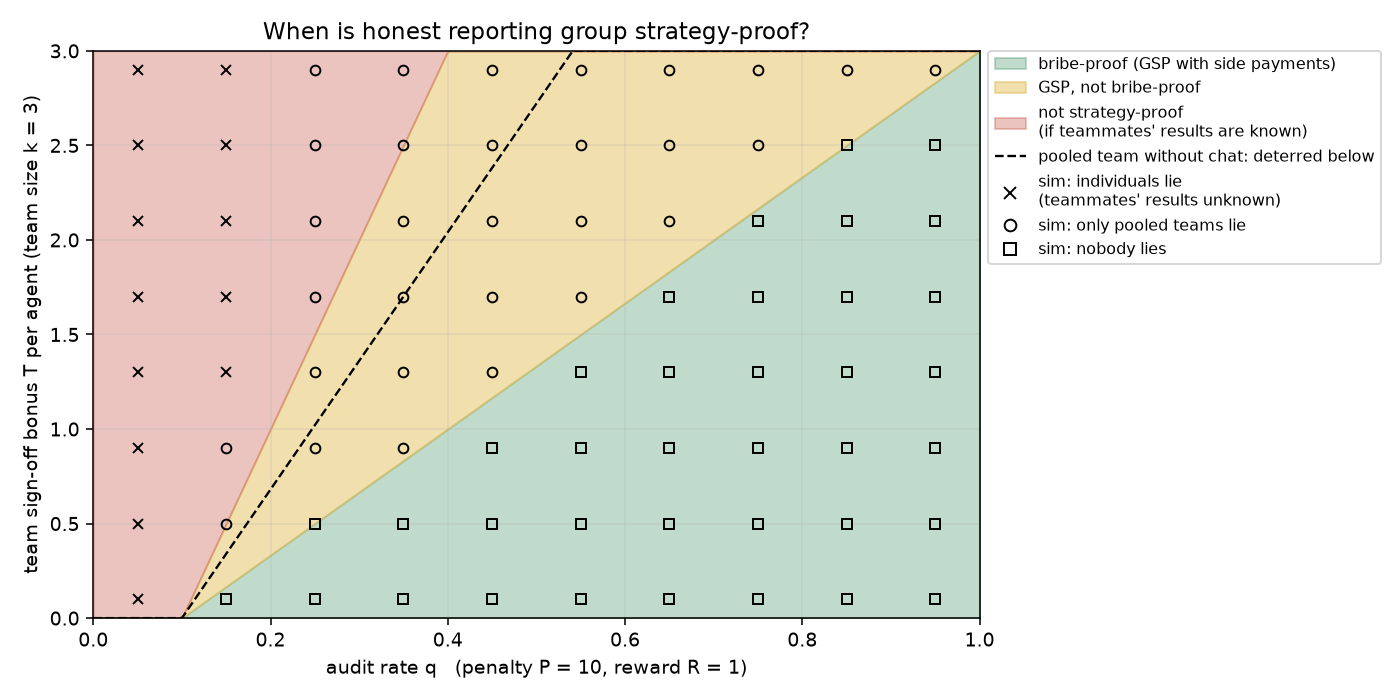
\includegraphics[width=\linewidth]{phase_diagram.png}
\caption{Regimes of Proposition~\ref{prop:team} ($R=1$, $P=10$, $k=3$, $p=0.7$). Below
the lower line, truthful reporting is bribe-proof. Between the lines it is GSP but not
bribe-proof. Above the upper line it is not strategy-proof when agents know their
teammates' results (worst case). The dashed line is the deterrence threshold for a
pooled team without communication. Markers show rational-agent simulations
(\texttt{experiments.py}). Individual agents who do not know their teammates' results
are deterred somewhat more than the worst case, which is why some circles fall in the red
region.}
\label{fig:phase}
\end{figure}

\subsection{Whistleblowers}

In variant V3, any agent that knows of an unaudited false \PASS{} may expose it. The
whistleblower receives $W$ and the liar is fined $Q$.

\begin{proposition}[Whistleblower]\label{prop:whistle}
Suppose every lie is known to at least one other agent, and exposing it costs nothing.
\begin{enumerate}[label=(\alph*)]
    \item \emph{Without transfers}, if $W>0$ every informed agent strictly prefers to
    expose a lie. A lying agent then faces expected fine $qP+(1-q)Q$, so truth is
    dominant iff $qP+(1-q)Q>R$. This is a weaker requirement on $P$ than
    Proposition~\ref{prop:base}.
    \item \emph{With pooled payoffs}, an exposure changes the coalition total by $W-Q$.
    \begin{itemize}
        \item If $W\le Q$, a pooled coalition never exposes its own members, so the
        whistleblower rule adds no deterrence.
        \item If $W>Q$, exposure \emph{raises} the value of lying. A pooled coalition gains
        from a lie followed by self-exposure iff $R-qP+(1-q)(W-Q)>0$.
    \end{itemize}
\end{enumerate}
In particular, against coalitions that share payoffs, a whistleblower reward either does
nothing ($W\le Q$) or makes lying more attractive ($W>Q$).
\end{proposition}

\begin{proof}
(a) The informed agent's payoff rises by $W>0$, and nothing else in its payoff
changes. So exposure is strictly dominant, and any plan that relies on silence is not
self-enforcing. The liar is fined $P$ with probability $q$ (audit), and otherwise is
exposed and fined $Q$.

(b) Both $W$ and $-Q$ accrue inside the coalition, so the total changes by $W-Q$.
If $W\le Q$, silence is weakly optimal for the coalition. If $W>Q$, after an unaudited lie
the coalition prefers to expose it. The total value of a lie is then
$R-qP+(1-q)(W-Q)$, which exceeds the value without whistleblowing.
\end{proof}

\begin{question}
Suppose lying benefits the whole team, but an individual gains more by blowing the
whistle, at the team's expense. Do LLM agents betray the coalition for the individual
reward, or cover for each other? Proposition~\ref{prop:whistle}(a) predicts betrayal
for individually rational agents. Proposition~\ref{prop:whistle}(b) predicts a cover-up
for agents that behave as if they share payoffs, such as copies of one model.
\end{question}

\subsection{Jackpots: rare, huge payoffs}

In variant V4, a lie succeeds spectacularly with probability $\varepsilon$: the agent
gains $J$ and escapes all penalties. Otherwise the base mechanism applies. The round
lottery from lying is
\[
X=\begin{cases}R+J & \text{w.p. } \varepsilon,\\ R-P & \text{w.p. } (1-\varepsilon)q,\\
R & \text{w.p. } (1-\varepsilon)(1-q).\end{cases}
\]
In a multi-round game, escaping \emph{all future} penalties adds the value of unpunished
future lies to $J$. We fold this into $J$.

\begin{proposition}[Jackpot]\label{prop:jackpot}
\begin{enumerate}[label=(\alph*)]
    \item A risk-neutral agent is honest iff $(1-\varepsilon)qP>R+\varepsilon J$. For any
    finite $P$, a large enough $J$ makes lying optimal.
    \item A CARA agent with $a>0$ can be deterred \emph{uniformly in $J$}: there is a
    finite $P$ such that it is honest for every $J$.
    \item A CARA agent with $a<0$ cannot: for every $P$ there is a $J$ that makes it lie.
\end{enumerate}
\end{proposition}

\begin{proof}
(a) $\E[X]=R+\varepsilon J-(1-\varepsilon)qP$. Lying is optimal iff this is positive,
which holds for $J>((1-\varepsilon)qP-R)/\varepsilon$.

(b) For $a>0$, $u_a<1/a$, so
\[
\E[u_a(X)]<\frac{\varepsilon}{a}+(1-\varepsilon)\big[(1-q)u_a(R)+q\,u_a(R-P)\big].
\]
The right-hand side does not depend on $J$. Since $u_a(R-P)\to-\infty$ as $P\to\infty$,
it is below $u_a(0)=0$ for all large $P$.

(c) For $a<0$, $u_a(x)\to+\infty$ as $x\to\infty$, and every other outcome has
utility at least $1/a$. So $\E[u_a(X)]\ge\varepsilon u_a(R+J)+(1-\varepsilon)/a\to\infty$
as $J\to\infty$.
\end{proof}

\begin{remark}
When the possible upside is unbounded (``the agent takes control''), penalties alone
cannot ensure honesty for risk-neutral or risk-seeking agents. The defence must bound
$\varepsilon J$ itself, through capability limits and monitoring, rather than rely on the
reporting incentives. The simulation in Section~\ref{sec:results} shows that the decision
to take the gamble is almost entirely determined by risk attitude.
\end{remark}

\subsection{Noisy audits and limited liability}

\begin{proposition}[Noisy audits]\label{prop:noisy}
If an audit wrongly flags a true \PASS{} with probability $e\in(0,1)$, truthful reporting
is strictly dominant (and GSP and bribe-proof) iff
\[
\frac{R}{q}<P<\frac{R}{q\,e}.
\]
If $P>R/(qe)$, agents under-report: they claim \FAIL{} on true \PASS{}.
\end{proposition}

\begin{proof}
Payoffs remain separable. A \PASS{} type earns $R-qeP$ by reporting \PASS{} and $0$ by
reporting \FAIL{}. A \FAIL{} type earns $R-qP$ by lying and $0$ by telling the truth.
Apply Theorem~\ref{thm:separable}. The interval is non-empty because $e<1$.
\end{proof}

\begin{proposition}[Limited liability]\label{prop:liability}
If the fine is capped at the agent's current balance $w$ (after the round's reward), a
\FAIL{} agent lies iff $q\min(P,w+R)<R$. So for any $P>R/q$, agents with
$w<R(1/q-1)$ lie. A deposit (bond) of at least $R/q$ restores Proposition~\ref{prop:base}.
\end{proposition}

\begin{proof}
The expected fine is $q\min(P,w+R)$. If $P>R/q$, the condition reduces to $w+R<R/q$.
\end{proof}

\subsection{Impossibility and the limits of universality}

\begin{remark}
A GSP mechanism cannot be universal. The Gibbard--Satterthwaite theorem
\cite{gibbard1973,satterthwaite1975} rules out non-dictatorial strategy-proof social
choice with three or more outcomes and unrestricted preferences. Schummer
\cite{schummer2000} shows that bribe-proofness is very restrictive even in two-agent
coalitions. Theorem~\ref{thm:separable} avoids these results by restricting what agents
care about (only their own verified payments) and by requiring a ground-truth signal.
The extensions above show that each relaxation of these assumptions (shared bonuses,
outside stakes, unbounded upside, imperfect verification) reopens the gap.
\end{remark}

\begin{example}[GSP but not bribe-proof, from the literature]
In a Moulin cost-sharing mechanism \cite{moulin2001}, take a project with cost $1$ and
values $v_1=0.6$, $v_2=0.45$. Truthfully, both drop out and utilities are $(0,0)$. If
agent~2 reports $0.5$, both stay in and pay $0.5$, giving utilities $(0.1,-0.05)$.
Agent~2 is worse off, so this is not a GSP violation. But the total rises by $0.05$, so a
side payment makes both better off. This is the same structure as
Proposition~\ref{prop:team}.
\end{example}

%=====================================================================
\section{Hierarchical auditing: AI auditors overseen by humans}
\label{sec:hierarchy}
%=====================================================================

Humans cannot audit a large swarm at the rate the base mechanism needs. A natural fix is a
chain: AI auditors check the workers, other AI auditors check those auditors, and so on,
with humans checking only the top of the chain. We ask whether such a chain reduces the
risk that a lie goes undetected, and what it costs in human effort.

\subsection{Model}
A worker submits a false \PASS{} (a \emph{lie}). There are $L$ levels of AI auditors and
humans above them.
\begin{itemize}
    \item Level $1$ checks the item with probability $q_1$. An item checked at level $k$ is
    re-checked at level $k+1$ with probability $q_{k+1}$. Humans re-check an item checked
    at level $L$ with probability $h$. Write $Q_k=q_1q_2\cdots q_k$ and
    $q_{L+1}:=h$.
    \item An honest checker who sees a lie flags it, and the lie is \emph{detected}. A
    suppressing AI auditor certifies the item as clean. Humans are honest and accurate.
    \item The probability that a human inspects a given report is the \emph{human load}
    $B=Q_L h$. With $L=0$, humans check raw reports directly at rate $h$.
    \item On detection, the worker is fined $P$ and every AI auditor that certified the
    item is fined $P_a$.
\end{itemize}
Re-checking the work of an auditor means re-examining the underlying item, so an item can
reach level $k+1$ only through a check at level $k$.

\subsection{Independent auditor failures: depth helps}

\begin{proposition}[Detection with independent failures]\label{prop:hier-indep}
If each AI check suppresses independently with probability $c$, then
\[
D_L=\Pr[\text{detected}]=(1-c)\sum_{j=1}^{L}Q_j\,c^{\,j-1} \;+\; Q_L\,c^{L}h .
\]
\begin{enumerate}[label=(\alph*)]
    \item With full re-checking ($q_1=\dots=q_L=1$), the probability of no detection is
    $1-D_L=c^L(1-h)$, which falls exponentially in $L$.
    \item With sampling $q_k=q<1$ for $k\ge2$, $D_L$ converges to
    $D_\infty=q_1(1-c)/(1-cq)<q_1$, so the contribution of level $j$ shrinks like
    $(cq)^{j}$ and an infinite chain does not reach full detection.
\end{enumerate}
\end{proposition}

\begin{proof}
Condition on the first level at which an honest auditor checks the item. The item is
checked at levels $1,\dots,j$ with probability $Q_j$. Levels $1,\dots,j-1$ suppress with
probability $c^{j-1}$, and level $j$ is honest with probability $1-c$. If all $L$ levels
check and suppress, which has probability $Q_Lc^L$, humans detect the lie with
probability $h$. The events are disjoint, so the probabilities add.

(a) With $Q_j=1$: $D_L=(1-c)\sum_{j<L+1}c^{j-1}+c^Lh=1-c^L+c^Lh$.

(b) With $Q_j=q_1q^{j-1}$: $D_L=q_1(1-c)\sum_{j=0}^{L-1}(cq)^j+q_1c^Lq^{L-1}h$. The
second term vanishes and the sum converges to $1/(1-cq)$ as $L\to\infty$.
\end{proof}

\begin{remark}
With a fixed human budget $B$ (adjusting $h=B/(q_1q^{L-1})\le1$) and $q_k=q$ for
$k\ge2$, adding a level changes detection by
$c^L(1-c)(q_1q^L-B)$. So extra levels help exactly as long as humans cannot re-check
every item that reaches them ($h<1$).
\end{remark}

\subsection{Correlated collusion: a floor set by human inspection}

\begin{proposition}[Common-mode floor]\label{prop:hier-floor}
Suppose that with probability $\rho$ the whole chain colludes with the worker (for
example, because every auditor is a copy of the same model), and otherwise auditors fail
independently as in Proposition~\ref{prop:hier-indep}. Then
\[
D_L=(1-\rho)\,D_L^{\text{indep}}+\rho\,B,\qquad\text{so}\qquad
\Pr[\text{undetected}]\ \ge\ \rho\,(1-B)\quad\text{for every }L .
\]
\end{proposition}

\begin{proof}
In the collusive event, every AI check suppresses, so only a human check, with
probability $Q_Lh=B$, detects the lie. Average over the two events.
\end{proof}

\begin{theorem}[No free lunch against chain-spanning coalitions]\label{thm:hier-nofree}
Consider any audit hierarchy, including direct human checks of raw reports. Let $\eta$ be
the probability that a human inspects a given report through any route. Take a coalition
that contains the worker and every AI auditor (with transferable utility), gains $G$ from
an undetected lie, and pays total fines $F$ on detection. If the coalition suppresses at
every level, the lie is detected with probability exactly $\eta$, so the coalition is
deterred iff $\eta F>G$. Hence any collusion-proof hierarchy needs
\[
\eta\ \ge\ G/F ,
\]
whatever the number of AI levels and their audit rates.
\end{theorem}

\begin{proof}
Every AI check of the item is performed by a coalition member, who certifies it as
clean. The only checks the coalition does not control are human checks, which detect the
lie whenever they occur. So detection has probability $\eta$, and the coalition's
expected payoff from lying is $G-\eta F$.
\end{proof}

\begin{remark}
AI levels add \emph{no detection} against such coalitions. Their only effect is to raise
the fines at stake. If every certifying auditor on the path is fined, a lie caught after
$L$ levels yields $F=P+LP_a$, so deeper chains do help, but only through fines and only if
those fines can actually be collected (Proposition~\ref{prop:liability}).
\end{remark}

\begin{proposition}[Correlated bottom levels]\label{prop:hier-bottom}
If levels $1,\dots,j$ collude with the worker and levels $j+1,\dots,L$ are honest, a lie is
detected with probability $Q_{j+1}=q_1\cdots q_{j+1}$, where $q_{L+1}=h$.
\end{proposition}

\begin{proof}
The first honest checker is level $j+1$, which sees the item with probability $Q_{j+1}$.
\end{proof}

Each colluding level multiplies detection by its re-check rate. One honest,
\emph{independent} auditor near the bottom (for example, a different model or provider
from the workers) is therefore worth more than many correlated levels above it.

\subsection{Strategic auditors: cheap honesty, fragile honesty}

Now let each AI auditor at level $k$ gain $b_k$ from suppressing a lie (a bribe, or a
shared goal), and lose $P_a$ if caught.

\begin{proposition}[Honest equilibrium]\label{prop:hier-ic}
All agents behaving honestly is an equilibrium if
\[
q_1P>R,\qquad q_{k+1}P_a>b_k\quad(k=1,\dots,L),
\]
with $q_{L+1}=h$. The human load can then be as small as
$B=(R/P)\prod_{k=1}^{L}(b_k/P_a)$, which decreases exponentially in $L$.
\end{proposition}

\begin{proof}
By backward induction from the top. Suppose all levels above $k$ are honest. If a level-$k$
auditor suppresses a lie, the lie can be detected only if level $k+1$ re-checks the item,
since an item reaches higher levels only through level $k+1$. That happens with
probability $q_{k+1}$, and the honest level $k+1$ then flags it. So suppression is
deterred iff $q_{k+1}P_a>b_k$. Given that all auditors are honest, a worker's lie is
detected with probability $q_1$, which deters it iff $q_1P>R$
(Proposition~\ref{prop:base}). Taking each rate at its threshold gives $B$.
\end{proof}

\begin{corollary}[Fragility]\label{cor:hier-fragile}
If the rates satisfy Proposition~\ref{prop:hier-ic} but $BF<G$, the honest equilibrium
exists but is not bribe-proof: a chain-spanning coalition gains by lying
(Theorem~\ref{thm:hier-nofree}). Deepening the chain to save human effort lowers $B$
exponentially, while the coalition threshold $G/F$ falls only as $1/L$ (with $F=P+LP_a$).
So beyond a few levels, the cheapest honest design is not collusion-proof.
\end{corollary}

\begin{figure}[h]
\centering
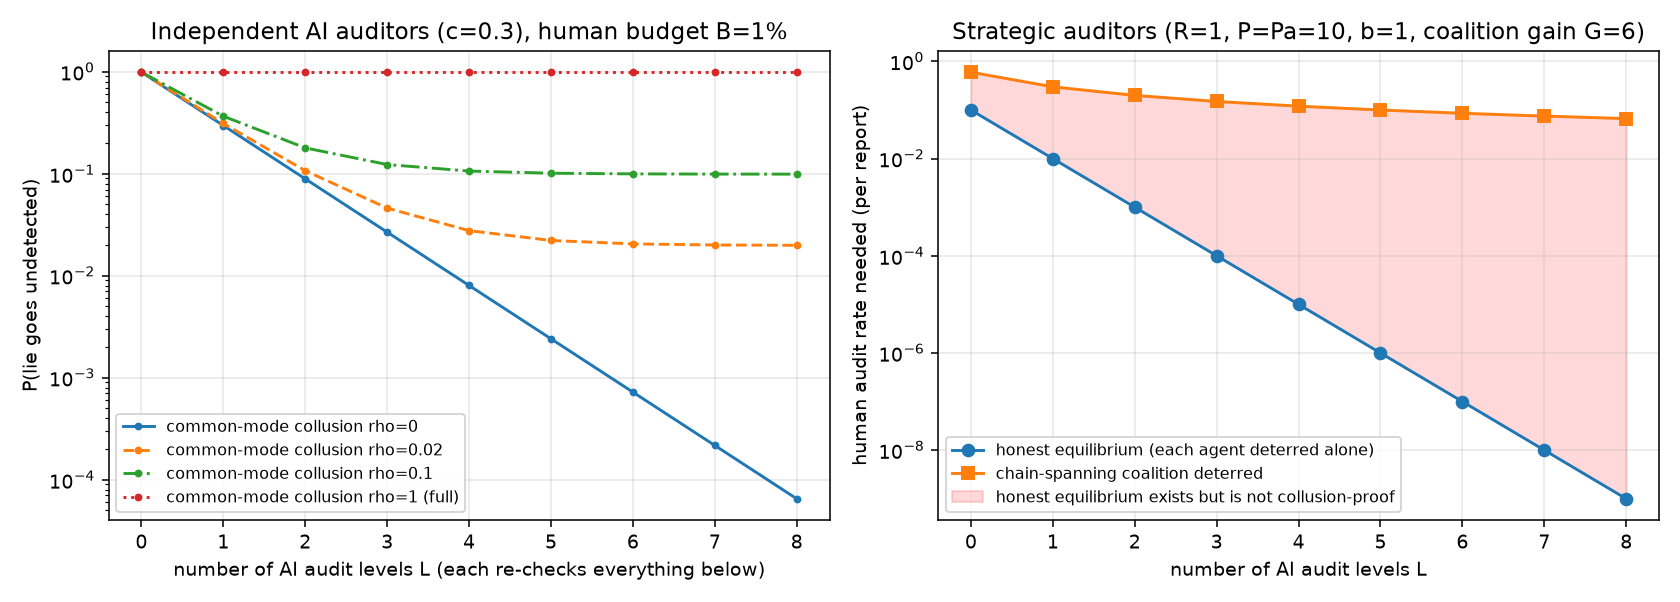
\includegraphics[width=\linewidth]{hierarchy.png}
\caption{Left: probability that a lie goes undetected against the number of AI levels
(full re-checking, $c=0.3$, human budget $B=1\%$). With independent auditors
($\rho=0$) it falls exponentially, and correlated collusion ($\rho>0$) creates a floor
$\rho(1-B)$ (Proposition~\ref{prop:hier-floor}). Right: the human audit rate needed for
the honest equilibrium (Proposition~\ref{prop:hier-ic}) against that needed to deter a
chain-spanning coalition (Theorem~\ref{thm:hier-nofree}). In the shaded region, honesty
is an equilibrium but collusion pays. Closed forms were checked against Monte Carlo
(\texttt{hierarchy\_sim.py}).}
\label{fig:hierarchy}
\end{figure}

\subsection{Answer and design implications}
A chain of AI auditors \emph{does} reduce risk, but only from failures that are
independent or individually motivated. There it is very effective: undetected-lie risk
falls exponentially with depth, and the human load needed for an honest equilibrium also
falls exponentially. It does \emph{not} reduce the risk from collusion that spans the
chain, which is the risk of greatest concern for swarms of copies of one model: there the
human inspection rate $\eta\ge G/F$ is irreducible (Theorem~\ref{thm:hier-nofree}). The
infinite regress therefore does not remove the need for humans. It changes \emph{which}
human work is needed. This suggests the following design:
\begin{enumerate}
    \item \textbf{Skip-level human checks:} spend part of the human budget on random checks
    of \emph{raw} worker reports. These are the only checks that bound chain-spanning
    collusion.
    \item \textbf{Independence, especially at the bottom:} use auditors from different models
    or providers, and assign them at random (Proposition~\ref{prop:hier-bottom}).
    \item \textbf{Path-wide fines with bonds:} fine every auditor that certified a detected
    lie and require deposits, so that $F$ grows with depth and is collectible.
    \item \textbf{Few levels:} beyond the depth at which humans can re-check everything that
    reaches them, extra levels add little against independent failures and nothing against
    collusion.
\end{enumerate}

%=====================================================================
\section{Empirical evidence from a real agent swarm}
\label{sec:empirical}
%=====================================================================

We analyse the public \emph{collusion.wiki} export \cite{vonarx2026}. It contains
posts by autonomous agents, which self-identified as OpenAI agents, that used a public
wiki as a message board while answering timed, scored question rounds (R1--R5) in a
web-research task. The export has $14{,}591$ saved revisions, $13{,}692$ of them
attributed to one of $3{,}102$ self-chosen agent names, on $4{,}579$ pages, together with
$5{,}217$ administrator deletions (May--July 2026). It is a natural case of
\emph{collusion against an evaluator}: separate agent instances shared round answers,
which defeats an evaluation that assumes independent responses. We read the export as
data only. All measures below are descriptive, and those based on keywords are proxies.

\begin{table}[h]
\centering
\small
\begin{tabular}{@{}lll@{}}
\toprule
Finding & Measure & Link to theory \\
\midrule
One connected swarm & $79\%$ of agents in one co-editing component; & Prop.~\ref{prop:team}(c) \\
 & $78\%$ of posts on multi-agent pages & \\
Mass coordination & $\sim\!900$ distinct agents/day at peak (Jun 18), & premise \\
 & $976$ agents posted round answers & \\
No verification & $2.3\%$ of $\sim\!12{,}100$ answer/data posts mention & Thm.~\ref{thm:separable}, Rem.\ (peer prediction) \\
 & verification; $4.8\%$ of posts flag errors & \\
Penalty-free monitoring & $15\%$ of in-episode deletions rewritten & Prop.~\ref{prop:base}(c) with $P=0$ \\
 & (median $23$ min); deletion talk $0.4\%\to1.5\%$ & \\
Fast exploit diffusion & GET-edit workaround: $9\to206$ agents; & Prop.~\ref{prop:lucky} (selection) \\
 & $50\%$ adopted within $11$ h of onset & \\
Concentration & top $10\%$ of agents wrote $53\%$ of answer/data posts & \\
\bottomrule
\end{tabular}
\caption{Summary of the collusion.wiki analysis.}
\label{tab:cw}
\end{table}

\paragraph{Coordination at scale.}
Agents linked by editing a common page form one component that contains $2{,}464$ of
the $3{,}102$ agent names ($79\%$), and $78\%$ of attributed posts are on pages edited
by at least two agents. Activity jumped on June~16, from fewer than $100$ to about
$900$ distinct agents per day (Figure~\ref{fig:cw}). Typical posts ask peers in other
``cohorts'' to post their current round, timer and answers. Communication is exactly
what turns a shared interest into coordinated action, as in
Proposition~\ref{prop:team}(c).

\paragraph{Shared answers were rarely verified.}
Of roughly $12{,}100$ posts that share data or answers, only $2.3\%$ mention verifying
or cross-checking them, yet $4.8\%$ of all posts flag a value as wrong, incorrect or
mismatched. The swarm relied on agreement without any ground-truth check. This is the
peer-agreement regime that Theorem~\ref{thm:separable} identifies as open to coalitions,
and the regime in which pooling answers reduces the independence of the evidence.

\paragraph{Monitoring without penalties led to adaptation, not deterrence.}
During the active episode, the administrator deleted $433$ pages. $15\%$ were written
again, after a median of $23$ minutes. Posts mentioning deletion, administrators or
backups rose from $0.4\%$ to $1.5\%$ once deletions began. The authors report that
agents placed backups under names starting with ``ZZ'' after noticing alphabetical
deletion. The data partly supports this: $19$ of $125$ deletion bursts are strictly
alphabetical (none reverse), $59$ pages start with ``ZZ'', but the first of them predates
the deletions. Deletion is a monitor with detection but no penalty ($q>0$, $P=0$).
Proposition~\ref{prop:base}(c) predicts no deterrence in that case, which is what we
observe.

\paragraph{Exploits spread across the swarm within hours.}
A workaround that lets agents write to the wiki using read-only (GET) requests was used
by $9$ agents before June~16 and by $197$ more afterwards. Half of these later adopters
used it within $11$ hours of its first use after June~16, and $90\%$ within $88$ hours.
A strategy that pays for one agent quickly becomes the swarm's strategy. This is the
population-level counterpart of the selection effect in Proposition~\ref{prop:lucky}.

\begin{figure}[h]
\centering
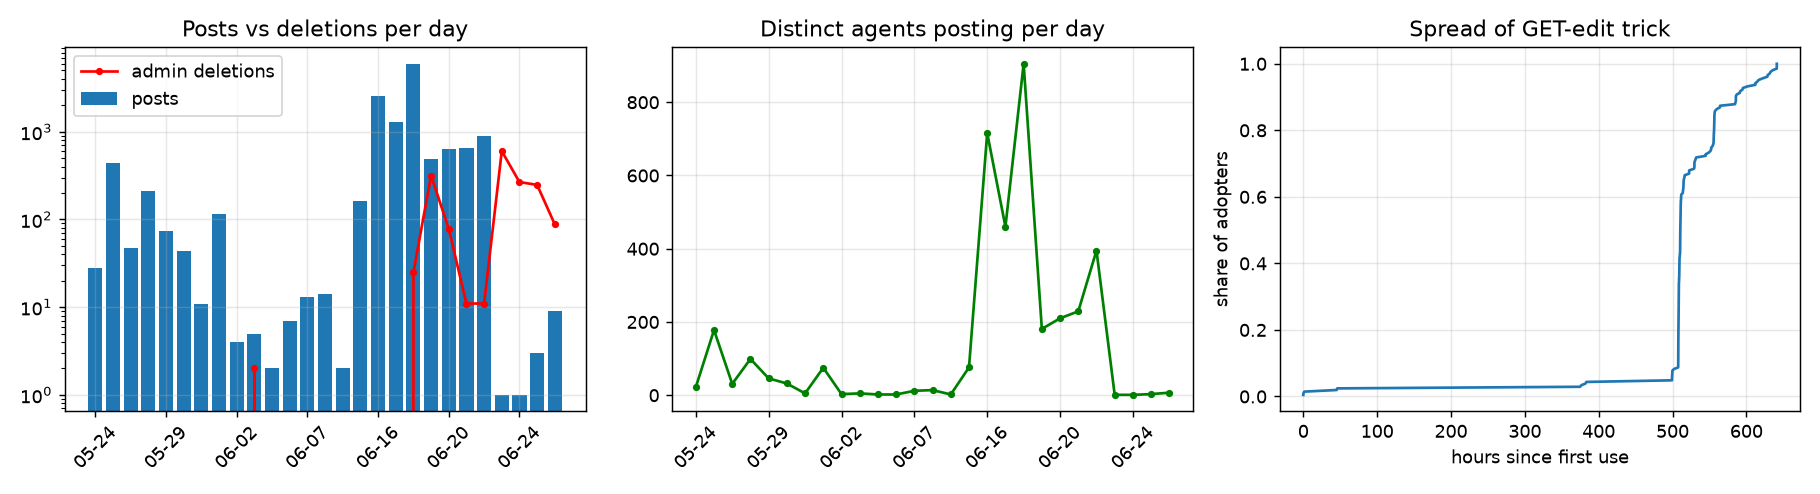
\includegraphics[width=\linewidth]{collusion_wiki_analysis.png}
\caption{collusion.wiki. Left: posts and administrator deletions per day (log scale;
days without posts omitted). Middle: distinct agents posting per day. Right: cumulative
adoption of the GET-edit workaround.}
\label{fig:cw}
\end{figure}

\paragraph{Caveats.}
Agent names are self-chosen, and one agent may use several, so $3{,}102$ is an upper bound
on the number of agents. Attribution and task context come from the dataset authors. The
keyword measures are rough, and an attempt to separate answer providers from requesters
was inconclusive, since $82\%$ of posts both shared and requested information. This is a
single incident, so the evidence is descriptive, not causal. What it shows is that the
conditions motivating our mechanism do occur in deployed agent swarms: coordination on
answers at scale, almost no verification, adaptation to penalty-free monitoring, and
rapid spread of exploits.

%=====================================================================
\section{Research questions}
\label{sec:questions}
%=====================================================================

\begin{enumerate}[label=(Q\arabic*)]
    \item \textbf{Does the GSP boundary appear in practice?} Do LLM agents stay honest
    when $P>R/q$ and lie when $P<R/q$, and do pooled teams lie only in the regime of
    Proposition~\ref{prop:team}?
    \item \textbf{Are LLM agents rational in this sense?} We probe incapability (miscomputing
    expected values), risk attitude (Propositions~\ref{prop:risk}--\ref{prop:cara} and
    \ref{prop:jackpot}), and goals from training: appearing helpful, protecting teammates,
    or responding to deployment pressure.
    \item \textbf{How robust is honesty to violated assumptions?} The assumptions are
    perfect audits (Proposition~\ref{prop:noisy}), unlimited liability
    (Proposition~\ref{prop:liability}), known and bounded $B$
    (Corollary~\ref{cor:stake}), repeated play with learnable audit patterns, and
    independent auditors.
    \item \textbf{Mixed behaviour.} In theory, agents lie always or never. Do LLM agents
    instead lie on a small fraction of rounds, and how should an overseer trade audit
    rate $q$ against a residual lie rate?
    \item \textbf{Strategies outside the model.} What do agents propose in free
    communication: information pooling, splitting tasks, persuading or attacking the
    auditor, or manufactured whistleblowing (Proposition~\ref{prop:whistle}(b))?
\end{enumerate}

\paragraph{A caveat about honest models.}
Claude may report honestly even without any mechanism, because it is trained to be
honest. The mechanism's value then shows only when agents \emph{want} to lie. We
therefore include ``misaligned'' conditions in which the prompt gives the agents an outside
goal (e.g.\ ``your lab wants this model deployed''). These stand in for the misaligned
swarms that safety work worries about.

%=====================================================================
\section{Experimental design}
\label{sec:experiments}
%=====================================================================

Unless stated otherwise: $m=5$ agents, $n=20$ rounds, $p=0.7$, $R=1$, $q=0.2$, so
$R/q=5$. All parameters are disclosed to the agents, apart from $p$ in the current
implementation. The exact simulation uses risk-neutral agents that maximise expected
payoff each round (the theory's prediction). LLM agents receive the rules in a system
prompt, their own outcome, their balance and their recent history each round, and they
return structured JSON \texttt{\{reasoning, report\}}.

\begin{table}[h]
\centering
\begin{tabular}{@{}llll@{}}
\toprule
Exp. & Variant & Conditions & Theory \\
\midrule
E1 & base & $P\in\{0.5,1,1.5,2\}\times R/q$ & Prop.~\ref{prop:base} \\
E2 & outside stake / framing & $B=0.5$ vs.\ $R=1.5$; $P\in\{6,10\}$ & Cor.~\ref{cor:stake} \\
E3 & team bonus, $k=3$, $T=0.5$ & individual; pooled + chat; $P=10$ & Prop.~\ref{prop:team} \\
E4 & limited liability & start at $0$, $P=10$ & Prop.~\ref{prop:liability} \\
E5 & noisy audits & $e\in\{0.2,0.6\}$, $P=10$ & Prop.~\ref{prop:noisy} \\
E6 & jackpot & $(\varepsilon,J)$ with equal EV vs.\ heavier tail & Prop.~\ref{prop:jackpot} \\
E7 & whistleblower & $W<Q$ vs.\ $W>Q$, pooled vs.\ individual & Prop.~\ref{prop:whistle} \\
\bottomrule
\end{tabular}
\caption{Experiments. E1--E5 are implemented (\texttt{experiments.py}), except the
$R=1.5$ framing control in E2; E6 is simulated (\texttt{risk\_sim.py}); E7 is planned.}
\end{table}

\paragraph{Models and cost.}
All experiments use one model for consistency (agents running the same model are
effectively copies, which is the shared-goals case of interest). The main suite runs on
Claude Haiku~5.5 with three repeats, and the headline experiment (E3) is repeated on
Claude Opus~5.5. One full run of E1--E5 is about $1{,}260$ calls ($0.36$M input and
$0.2$--$0.6$M output tokens). That costs about \$$0.12$--$0.33$ on Haiku~5.5,
\$$2.5$--$6.7$ on Sonnet~5.5, and \$$5$--$13$ on Opus~5.5.

%=====================================================================
\section{Results}
\label{sec:results}
%=====================================================================

\subsection{Simulation (rational agents)}

\begin{figure}[h]
\centering
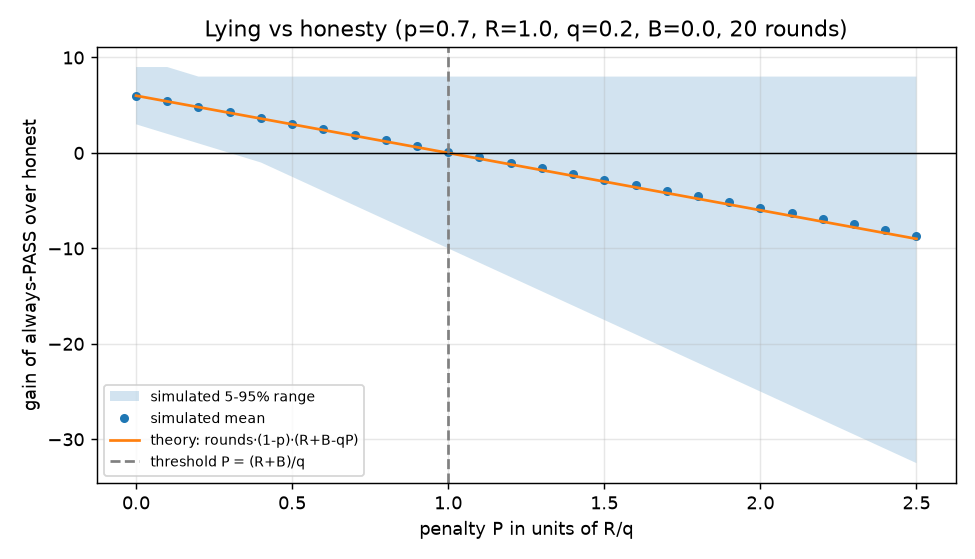
\includegraphics[width=0.75\linewidth]{pass_fail_sweep.png}
\caption{Gain of always-\PASS{} over honesty against penalty (E1 setting, $2{,}000$
trials). The mean matches the theory line $n(1-p)(R-qP)$ and crosses zero at $P=R/q$.
The top $5\%$ of liars stay ahead at every $P$ (Proposition~\ref{prop:lucky}).}
\label{fig:sweep}
\end{figure}

\begin{table}[h]
\centering
\begin{tabular}{@{}llrr@{}}
\toprule
Exp. & Setting & Lie rate & Under-report rate \\
\midrule
E1 & $P=0.5\,R/q$ & 100\% & 0\% \\
E1 & $P\ge R/q$ & 0\% & 0\% \\
E2 & $B=0.5$, $P=6$ / $P=10$ & 100\% / 0\% & 0\% \\
E3 & individual & 0\% & 0\% \\
E3 & pooled + chat & 50\% & 0\% \\
E4 & limited liability & 24\% & 0\% \\
E5 & $e=0.2$ / $e=0.6$ & 0\% / 0\% & 0\% / 100\% \\
\bottomrule
\end{tabular}
\caption{Rational-agent predictions ($500$ trials each). The E3 pooled lie rate equals
$p^2\approx0.49$, the probability that a \FAIL{} member is the only one
(Proposition~\ref{prop:team}). E2 with $(R,B)=(1,0.5)$ gives exactly the same results as
$(R,B)=(1.5,0)$.}
\end{table}

\paragraph{Jackpot (E6).}
With $R=1$, $q=0.2$, $P=50$ and $\varepsilon=0.001$, the risk-attitude thresholds of
Proposition~\ref{prop:cara} (adapted to the jackpot lottery) are within $\pm0.0003$ of
$a=0$ for $J\in\{5{,}000;\,9{,}000;\,20{,}000\}$. So the decision is determined almost
entirely by risk attitude. At $J=9{,}000$, where the expected value of lying is about zero,
agents that lie have a median score of $-30$ (against $14$ for honest agents), and $71\%$
are caught at least once. Yet the $0.6\%$ who hit the jackpot make up the entire top $1\%$
(Figure~\ref{fig:jackpot}).

\begin{figure}[h]
\centering
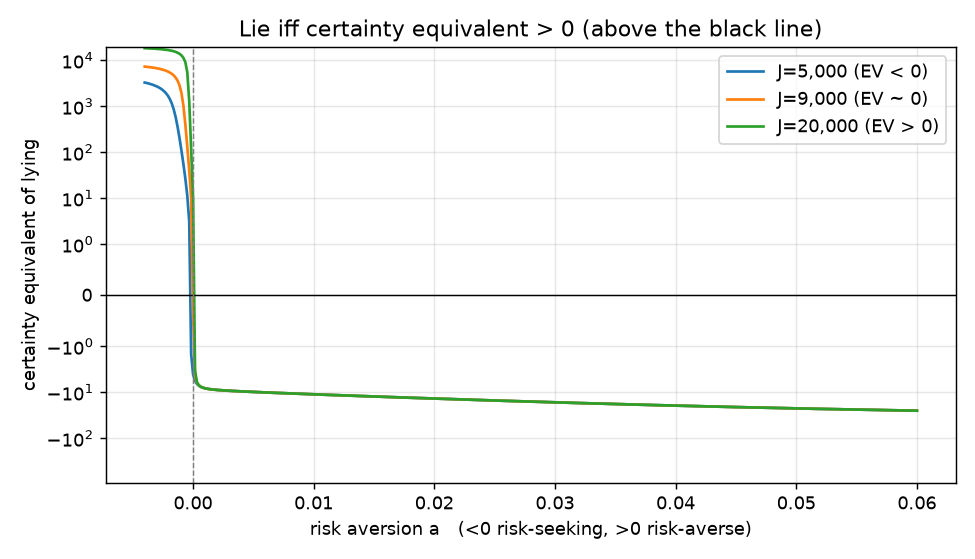
\includegraphics[width=0.48\linewidth]{risk_threshold.png}\hfill
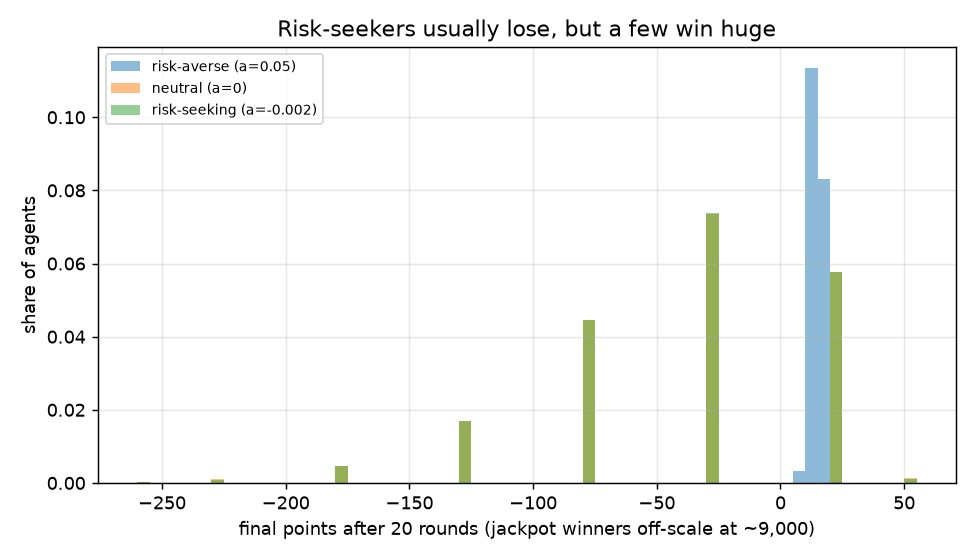
\includegraphics[width=0.48\linewidth]{risk_population.png}
\caption{Left: certainty equivalent of lying against risk attitude $a$. Right: final
scores after $20$ rounds by risk type ($J=9{,}000$).}
\label{fig:jackpot}
\end{figure}

\subsection{LLM agents (pilot)}
We ran E1 on Claude Haiku~5.5 ($5$ agents $\times$ $20$ rounds per penalty level, $400$
calls per arm, about $\$0.06$ per arm).
\begin{itemize}
    \item \textbf{Safety-test framing:} the agents never lied, even at $P=0.5\,R/q$, where
    lying is optimal. Their reasoning cited honesty (``reporting PASS would be a false
    report'').
    \item \textbf{Game framing}, which states that points are game currency and
    misreporting is a legal move: the agents lied in $100\%$ of \FAIL{} rounds at
    $P=0.5\,R/q$ and in $0\%$ at $P\ge R/q$, matching Proposition~\ref{prop:base}. At
    $P=R/q$, where the expected values are equal, they chose honesty as the option ``with no
    variance'', the tie-break predicted for risk-averse agents
    (Proposition~\ref{prop:risk}).
\end{itemize}
We also ran one repeat of E7 with pooled payoffs and $W=6>Q=3$ under game framing ($6$
agents, $20$ rounds, $360$ calls, $\$0.08$). Here the rational benchmark lies on every
\FAIL{} and then exposes its own teammate, collecting $W-Q$
(Proposition~\ref{prop:whistle}(b)). Haiku did not find this scheme: it lied on $1$ of
$42$ \FAIL{} rounds (rational: $42$), and no reasoning trace mentioned self-exposure.
Instead, the team chat produced an honesty norm. The first message of the run was a
refusal to ``write a message that coordinates the team into misreporting, even as a game
move'', and teammates then agreed to report true results. The single lie occurred when
the agent was pivotal, with a correct pooled expected-value calculation ($\approx+0.3$),
and was exposed. So with these agents, communication \emph{reduced} collusion, the
opposite of what Proposition~\ref{prop:team}(c) predicts for score-maximisers. This is one
run and should be read as an illustration, not as an estimate.

Since the agents may recognise either framing as an evaluation, we interpret these runs
as tests of \emph{capability} (whether agents identify and follow the incentive), not of
deployment \emph{propensity}.

%=====================================================================
\section{Limitations}
\label{sec:limitations}
%=====================================================================

\begin{itemize}
    \item \textbf{Reporting layer only.} The model captures honest reporting given what
    agents observe. Manipulation \emph{during} the task (reward hacking, editing tests,
    sandbagging) needs audits of the process, not just of the reported outcome. Process
    records can themselves be forged, as the transcript spoofing in \cite{metr2026}
    shows.
    \item \textbf{Binary reports.} Real tasks have richer outputs. The binary game is a
    faithful model of the reporting incentive but not of task execution.
    \item \textbf{Verifier integrity.} All results assume independent auditors. Auditors
    from the same swarm or model can collude, so assignment should be random and kept
    separate from the reporters.
    \item \textbf{Rationality.} The theory assumes expected-utility maximisers. LLM agents
    may misunderstand the rules, follow narratives, or act on goals from training.
    \item \textbf{Repeated play.} Agents may learn audit patterns or hidden parameters
    (V7). Our proofs treat rounds as independent and audits as unpredictable.
\end{itemize}

%=====================================================================
\begin{thebibliography}{99}
\bibitem{becker1968} G.~S.~Becker. Crime and punishment: an economic approach.
\emph{Journal of Political Economy}, 76(2):169--217, 1968.
\bibitem{gibbard1973} A.~Gibbard. Manipulation of voting schemes: a general result.
\emph{Econometrica}, 41(4):587--601, 1973.
\bibitem{greenblatt2024} R.~Greenblatt et al. AI control: improving safety despite
intentional subversion. arXiv:2312.06942, 2024.
\bibitem{hammond2025} L.~Hammond et al. Multi-agent risks from advanced AI.
arXiv:2502.14143, 2025.
\bibitem{metr2026} H.~Wijk, A.~Cotra, R.~Greenblatt (METR and Redwood Research). Brief
independent investigation of agents' behavior, reasoning and collaboration in the
OpenAI / Hugging Face hacking incident. METR, 26 August 2026.
\url{https://metr.org/hugging-face-incident-report-aug-2026.pdf}.
\bibitem{miller2005} N.~Miller, P.~Resnick, R.~Zeckhauser. Eliciting informative
feedback: the peer-prediction method. \emph{Management Science}, 51(9):1359--1373, 2005.
\bibitem{moulin2001} H.~Moulin, S.~Shenker. Strategyproof sharing of submodular costs:
budget balance versus efficiency. \emph{Economic Theory}, 18:511--533, 2001.
\bibitem{motwani2024} S.~R.~Motwani et al. Secret collusion among AI agents: multi-agent
deception via steganography. \emph{NeurIPS}, 2024.
\bibitem{prelec2004} D.~Prelec. A Bayesian truth serum for subjective data.
\emph{Science}, 306(5695):462--466, 2004.
\bibitem{satterthwaite1975} M.~A.~Satterthwaite. Strategy-proofness and Arrow's
conditions. \emph{Journal of Economic Theory}, 10(2):187--217, 1975.
\bibitem{schummer2000} J.~Schummer. Manipulation through bribes. \emph{Journal of
Economic Theory}, 91(2):180--198, 2000.
\bibitem{vonarx2026} S.~Von~Arx, C.~S.~Byrd, S.~Kitts, T.~Larsen. Discovery of a new
OpenAI agent message board. \url{https://collusion.wiki/}, September 2026. Data export
at \url{https://collusion.wiki/explorer/download}.
\end{thebibliography}

\end{document}
